\documentclass{beamer}
\usetheme{manhattan}  % Now it's a beamer presentation with the Manhattan College theme!

\usepackage{url}
\usepackage{graphicx}
\usepackage{fancyvrb}
\usepackage{MnSymbol, amsthm, amsfonts, amsmath, amssymb, amsxtra}

\newcommand{\Z}{\mathbb{Z}}
\beamertemplatenavigationsymbolsempty


% Make a new command that will make a new subsection and a frame with the same title
\newcommand{\fst}[2]{\subsection{#1}\frame{\frametitle{#1} #2}}
\newcommand{\ft}[2]{\frame{\frametitle{#1} #2}}

% ~ instead of spaces prevents linebreaks
\title{Using~Kolmogorov~Complexity~to~Make~All~the~Art}
\author{Jonathan Langke and Peter Boothe}
\date{6 April 2013}
\institute[Manhattan College]{
    \url{jlangke.student@manhattan.edu}\\
    Computer Engineering '13 \\
    ~\\
    \url{peter.boothe@manhattan.edu}\\
    Computer Science\\
    ~\\
    Manhattan College}

\begin{document}
\frame{\titlepage}

\section{What is Art?}

\fst{Art!}{
	\begin{center}
	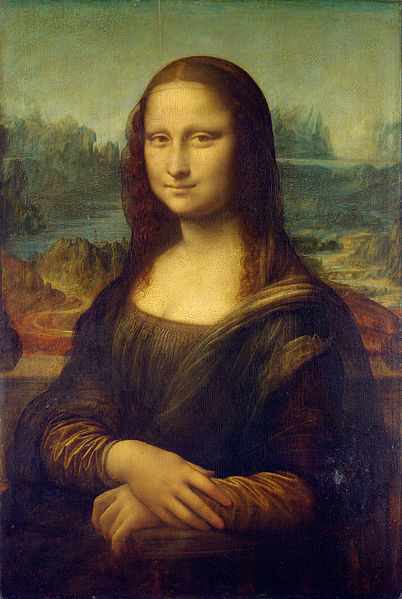
\includegraphics[height=2.5in]{monalisacolor.jpg}
	\end{center}
}

\ft{Art!}{
	\begin{center}
	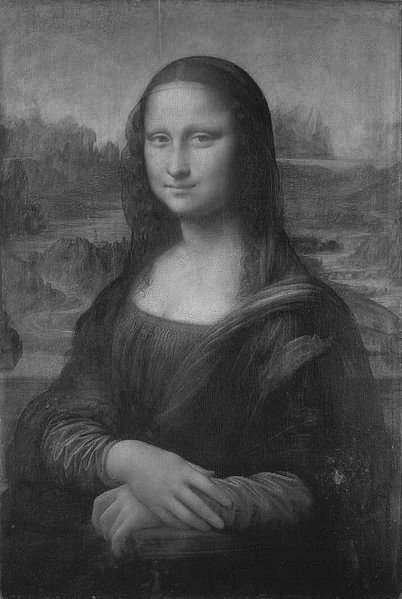
\includegraphics[height=2.5in]{monalisagray.jpg}
	\end{center}
}

\ft{Art!}{
	\begin{center}
	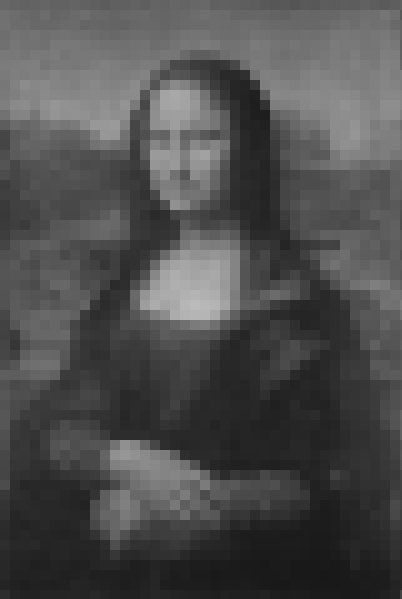
\includegraphics[height=2.5in]{monalisagraypixels.jpg}
	\end{center}
}

\ft{Art!}{
	\begin{center}
	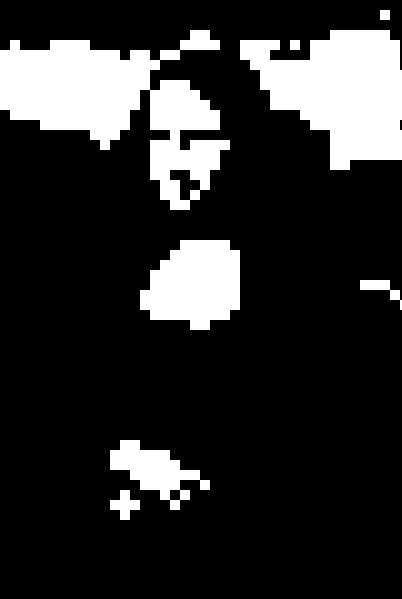
\includegraphics[height=2.5in]{monalisabwpixels.jpg}
	\end{center}
}

\fst{Int $\times$ Int $\to$ Bool}{
	\begin{itemize}
		\item A restricted form of digital art
		\item black and white pixels on a grid
		\item black is ``true'', white is ``false''
		\item each pixel's color is a function of its grid coordinates
		\item art is a function mapping $(\Z\times \Z)$ to $\{ true, false \}$
	\end{itemize}

	\pause
	\begin{center}\LARGE{Some art is more complex than other art}\end{center}
}
\fst{Example}{
\begin{centering}
\begin{tabular}{p{2in}   p{2in}}
(x $<$ y) &
(((1 + (1 + 1)) $<$  (x * y)) and 
		      ((x + 1) $<$ (y * (1 + 1)))) \\
\pause\\
3 symbols & 19 symbols\\
\end{tabular}
\pause
\begin{tabular}{p{2in}   p{2in}}
	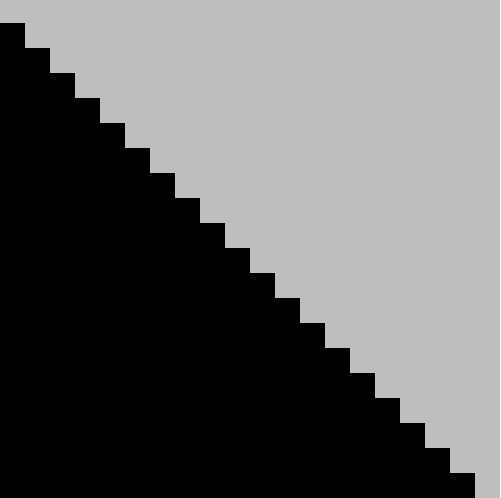
\includegraphics[width=1.5in]{simple.png} &
	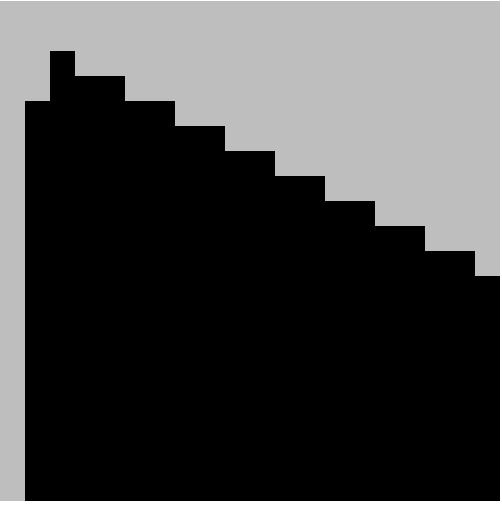
\includegraphics[width=1.5in]{complex.png} \\
\end{tabular}

($+x$ is to the right, $+y$ is down --- it's a computer graphics thing)
\end{centering}
}

\fst{Visual complexity}{
\begin{description}
	\item[Visual complexity] fuzzy and hard to define, but intuitive

	\item[Computational complexity] well defined, but complicated and (arguably) unintuitive
\end{description}

\vfill

\begin{center}
\LARGE{Perhaps visual complexity is correlated with computational complexity?}
\end{center}

\vfill
}

\section{Kolmogorov Complexity}

\fst{Complexity, quantified}{
	\begin{itemize}
		\item The complexity of an object is the size of the smallest program (a.k.a. formula) which outputs that object.
		\item That's Kolmogorov Complexity! ($KC$)
		\pause
		\item What programming language?\\
		\pause
		\textbf{Doesn't matter, they are all equivalent!}\\
		{\footnotesize (The $KC$ of an object in one language is equivalent to the $KC$ of that same object in another language, up to an additive constant.)}
		\pause
		\item What programming language?\\
		\pause
		\textbf{Racket.}
	\end{itemize}
}

\fst{Example}{
\begin{centering}
\begin{tabular}{p{2in}   p{2in}}
(x $<$ y) &
(((1 + (1 + 1)) $<$  (x * y)) and 
		      ((x + 1) $<$ (y * (1 + 1)))) \\
3 symbols & 19 symbols\\
	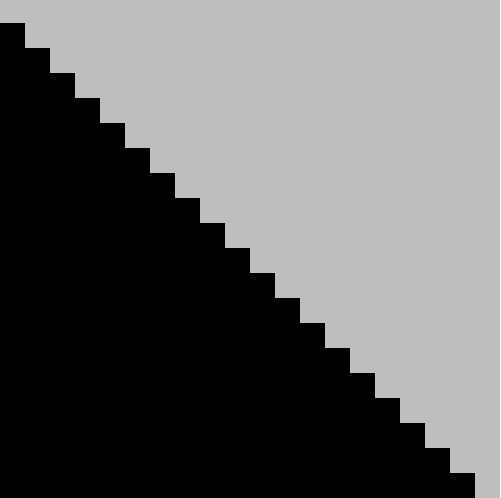
\includegraphics[width=1.5in]{simple.png} &
	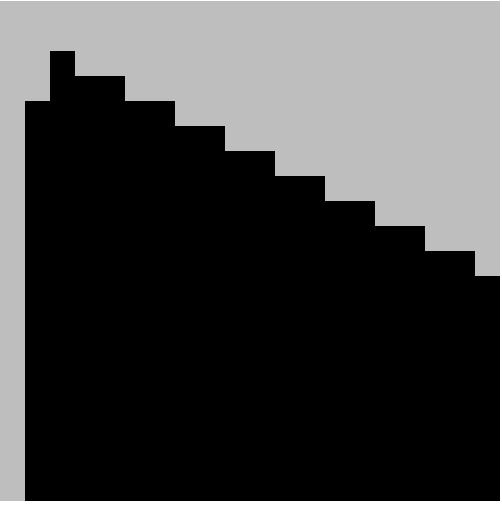
\includegraphics[width=1.5in]{complex.png} \\
Kolmogorov complexity of 3 &
Kolmogorov complexity of 19
\end{tabular}

\vfill

{\footnotesize (Remember: $+x$ is to the right, $+y$ is down)}
\end{centering}
}


\section{Logic Programming}

\fst{PROgramming with LOGic}{
	\begin{itemize}
		\item Specify relationships
		\item Computer generates objects which satisfy those relationships
		\item We used MiniKanren, a library for Racket\footnote{Racket is a descendant of Scheme and LISP} developed for this purpose
	\end{itemize}
}

\fst{MiniKanren}{
	\begin{itemize}
		\item A logic programming language/library for Racket.
		\item Specify relationships, e.g.:\\
			{\tt (def cousin \\
\hspace{.25in}($\lambda$ (p1 p2) \\
\hspace{.5in}(and (== (grandparent p1) (grandparent p2)) \\
\hspace{.9in}(!= (parent p1) (parent p2))))}
		\item When asked appropriately, MiniKanren will generate objects which satisfy a relation. e.g.:\\
			{\tt (run* (x) (cousin x 'JonathanLangke))}
	\end{itemize}
}

\section{All the Art}

\ft{}{
	\begin{center}
		
\includegraphics[width=3.5in]{alltheart.png}\\
		\url{http://hyperboleandahalf.blogspot.com/2010/06/this-is-why-ill-never-be-adult.html}
	\end{center}
}

\fst{Our Algorithm}{
	\begin{enumerate}
		\item Define what it means to be a ``well-typed'' (internally consistent, i.e. non-crashing) program of a particular size
		\item Generate, using MiniKanren, all well-typed programs up to a particular size
		\item Run each program to generate its corresponding image
		\item Record the smallest program which generates each image\\
~\\
		\pause
		\item PROFIT!
	\end{enumerate}
}

\fst{All the 2x2 Art}{
\begin{tabular}{r c l}
Formulae & Level & Pictures \\
\tiny{none} & 0 & empty \\
\tiny{(true), (false)} & 1 &
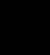
\includegraphics[width=.25in]{2x2/Shape1LVL1.png}~

\includegraphics[width=.25in]{2x2/Shape2LVL1.png} \\
\tiny{none} & 2 & empty \\
\tiny{(x $<$ 1), (y $<$ 1), (x $<$ y), (0 $<$ x), (0 $<$ y), (y $<$ x)} & 3 & 

\includegraphics[width=.25in]{2x2/Shape1LVL3.png}~

\includegraphics[width=.25in]{2x2/Shape2LVL3.png}~

\includegraphics[width=.25in]{2x2/Shape5LVL3.png}~

\includegraphics[width=.25in]{2x2/Shape6LVL3.png}~

\includegraphics[width=.25in]{2x2/Shape3LVL3.png}~

\includegraphics[width=.25in]{2x2/Shape4LVL3.png}\\
\tiny{(not (x $<$ y)), (not (y $<$ x))} & 4 & 

\includegraphics[width=.25in]{2x2/Shape2LVL4.png}~
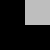
\includegraphics[width=.25in]{2x2/Shape1LVL4.png} \\
\tiny{((y + x) $<$ 1), ((y * x) $<$ 1), (0 $<$ (y + x)), (1 $<$ (y + x))} & 5 & 

\includegraphics[width=.25in]{2x2/Shape2LVL5.png}~
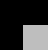
\includegraphics[width=.25in]{2x2/Shape1LVL5.png}~

\includegraphics[width=.25in]{2x2/Shape3LVL5.png}~

\includegraphics[width=.25in]{2x2/Shape4LVL5.png} \\
\tiny{none} & 6 & empty \\
\tiny{((y $<$ x) or (x $<$ y))} & 7 &

\includegraphics[width=.25in]{2x2/Shape1LVL7.png}\\
\tiny{(not ((y $<$ x) or (x $<$ y)))} & 8 &

\includegraphics[width=.25in]{2x2/Shape1LVL8.png}
\end{tabular}

\vfill

\begin{center}{\tiny (Remember: $+x$ is to the right, $+y$ is down)}\end{center}
}

\fst{Some Larger Art}{
\begin{center}
\begin{tabular}{r | c c c c c}
Art & 
\includegraphics[width=.4in]{YxY/4x8.png}&

\includegraphics[width=.5in]{YxY/5x7.png}&
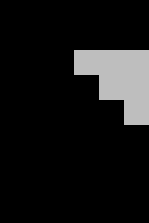
\includegraphics[width=.6in]{YxY/6x9.png}&

\includegraphics[width=.7in]{YxY/7x13.png}&

\includegraphics[width=.9in]{YxY/9x3.png}\\
\hline
Size & 4x8 & 5x7 & 6x9 & 7x13 & 9x3 \\
\hline
$KC$ & 7 & 7 & 6 & 6 & 5
\end{tabular}
\end{center}
}

\fst{References}{
    \bibliographystyle{plain}
    \bibliography{bib} 
}


\fst{What We Did}{ 
    \begin{enumerate}
        \item Defined what it meant to be an acceptable program
	\begin{enumerate}
		\item Built out of $<$, and, or, not, 0, 1, x, y, $+$, $*$
		\item Formula evaluates to true or false
	\end{enumerate}
        \item Defined art
	\begin{enumerate}
		\item Black and white pixel grid, corresponds to a boolean formula
		\item 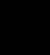
\includegraphics[width=.15in]{2x2/Shape1LVL1.png} ~
		
\includegraphics[width=.15in]{2x2/Shape2LVL1.png}
	\end{enumerate}
        \item Used MiniKanren to generate, from our constraints in step 1, all formulae of a given size
        \item Evaluated each formula (i.e. executed each program) to find its pictorial output.
	\begin{enumerate}
		\item When an output was produced multiple times, we chose the smallest formula
	\end{enumerate}
	\item Put it all together to discover the Kolmogorov Complexity of very small pieces of art.
    \end{enumerate}
\pause
        \hfill {\LARGE Any questions?}
    \color{white}{
        \cite{ReasonedSchemer}
        %\cite{SeasonedSchemer}
        %\cite{LittleSchemer}
        \cite{Yoo}
        \cite{Variadic}
    }
}
\end{document}
